\section{Base Model}
First, we set out to develop a base model. However, first, we had to decide which image size to use.
We chose an image size of 224x224, as this size seems to capture enough details. Also, many of the pretrained models uses the same image size, making our model more comparable to these.
Resizing the images has the effect of making training of the model significantly faster.

Next, we had to decide how many layers our model should have.
As the task is relatively simple, we decided to use 4 convolutional layers and 3 fully connected layers, including the binary output layer.
Since the input images are in color and 224x224 pixels, inputting that image directly into the fully connected layers would result in a $224\cdot224\cdot3 = 150528$ input size into the model. We would like to reduce this further, so the fully connected layers does not get an input of 150528. The convolution layers extract features, which makes it possible for the neural network to recognise a specific feature no matter where it is in the image, instead of having to learn that feature for every possible position in an image.

We use cross-entropy loss as our loss function since this loss function is a generally good and popular for classification tasks. We use Adam as the optimizer since it combines the strength of several other optimizers.

\#TODO: Mangler at beskrive activation function, kernel size og maxpooling


The base model is shown in Table \ref{tab:base_model}.
\begin{table}[H]
    \vspace*{-0.5cm}
    \centering
    \begin{tabular}{|l|c|c|c|c|}
    \hline
                & \textbf{Output}           & \textbf{Kernel}   & \textbf{MaxPooling}   & \textbf{Activation}   \\ 
                & \textbf{kernels/features} &                   &   &   \\ \hline
    Conv2D w/   & 32                        & 3x3                   & 2x2                   & ReLU                  \\ \hline
    Conv2D w/   & 64                        & 3x3                   & 2x2                   & ReLU                  \\ \hline
    Conv2D w/   & 128                       & 3x3                   & 2x2                   & ReLU                  \\ \hline
    Conv2D w/   & 256                       & 3x3                   & 2x2                   & ReLU                  \\ \hline
    Linear w/   & 256                       & -                     & -                     & ReLU                  \\ \hline
    Linear w/   & 128                       & -                     & -                     & ReLU                  \\ \hline
    Linear w/   & 2                         & -                     & -                     & -                     \\ \hline
    \end{tabular}
    \caption{Base Model.}
    \label{tab:base_model}
    \vspace*{-0.8cm}
\end{table}

We chose to train the model in 25 epochs with a learning rate of 0.001 as this generally is a good choice. A learning rate that is too small could result in a very slow learning process that might get stuck, and a too big learning rate could result in learning a suboptimal set of weights or an unstable learning process. Results of the base model after 25 epochs are shown in Figure \ref{fig:base_model_results}.
\begin{figure}[H]
    \vspace*{-0.7cm}
    \centering
    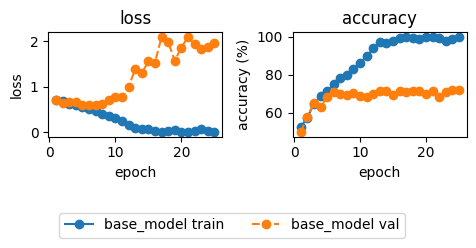
\includegraphics[width=0.4\textwidth]{figures/results_base_model.png}
    \caption{Base Model Results.}
    \label{fig:base_model_results}
    \vspace*{-0.7cm}
\end{figure}

Clearly, the base model is overfitting, therefore, we need to add some regularization to the model.